\documentclass[letterpaper,10pt,titlepage]{article}

\usepackage{graphicx}                                        
\usepackage{amssymb}                                         
\usepackage{amsmath}                                         
\usepackage{amsthm}                                          

\usepackage{alltt}                                           
\usepackage{float}
\usepackage{color}
\usepackage{url}

\usepackage{balance}
\usepackage[TABBOTCAP, tight]{subfigure}
\usepackage{enumitem}
\usepackage{pstricks, pst-node}

\usepackage{geometry}
\geometry{textheight=8.5in, textwidth=6in}

%random comment

\newcommand{\cred}[1]{{\color{red}#1}}
\newcommand{\cblue}[1]{{\color{blue}#1}}

\usepackage{hyperref}
\usepackage{geometry}

\def\name{Geoffrey Corey, MingChieh Chang, Ryan Susnjara, Raoul Aditya}

%pull in the necessary preamble matter for pygments output
\input{pygments.tex}

%% The following metadata will show up in the PDF properties
\hypersetup{
  colorlinks = true,
  urlcolor = black,
  pdfauthor = {\name},
  pdfkeywords = {cs411 ``operating systems'' kernel tools, scheduler},
  pdftitle = {CS 411 Project 1: Class Tools and Kernel Scheduling},
  pdfsubject = {CS 411 Project 1},
  pdfpagemode = UseNone
}

\begin{document}

%input the pygmentized output of mt19937ar.c, using a (hopefully) unique name
%this file only exists at compile time. Feel free to change that.
%\input{__mt19937ar.c.tex}
%\input{__project1.patch.tex}

\section{Design}
\label{Design Process & Implementation}
To implement the Round Robin (RR) and First In First Out (FIFO) schedulers in the Linux kernel, the group decided to not "reinvent the wheel." Since the real-time scheduler already had a RR and FIFO completed. However, with the code provided for the project, these algorithms have been removed. to remedy this, we diffed between the "vanilla" 3.0.4 kernel obtained from kernel.org against the provided 3.0.4 kernel files. The difference was in kernel\/sched.c and kernel\/sched\_rt.c. We created a patch that would add the missing functions and functionality back into the kernel. The basic flowchart is provided below.

\begin{center}
\includegraphics[width=4in]{design.eps}
\end{center}

\section{Code}
\label{Implementation Specific Code}
\input{__project1.patch.tex}

\end{document}
